\documentclass[11pt,a4paper]{article}
\usepackage[T1]{fontenc}
\usepackage[margin=2.3cm]{geometry}
\usepackage{amsmath,amssymb}
\usepackage{graphicx}
\usepackage[dvipsnames]{xcolor}
\usepackage{enumitem}
\usepackage[colorlinks=true,linkcolor=blue,urlcolor=blue]{hyperref}
\setlength{\parskip}{0.6em}
\setlength{\parindent}{0pt}
\begin{document}

\begin{center}{\LARGE\bfseries opencentripetal}\\[0.4em]{\large Design a banked curve that grips at speed, in three sessions.}\\[0.2em]\small PAN IIT OSS explainer \textbullet{} secondary school to diploma / undergraduate (levels 3-5)\end{center}

\section*{Why this exists}
Every car on a bend, every roller-coaster loop and every satellite is held on a curved path by an inward force. This explainer shows the mathematics of that force, using only algebra and a little trigonometry, so you can build it yourself.

\section*{The end goal}
Design a banked curve or roundabout that grips at speed. The end goal is to design a banked curve or roundabout that grips at speed: choosing a bank angle, knowing the safe speed range on dry and wet roads, and setting a speed limit with a margin. All models here are simplified teaching models and not a road design tool.

\section*{How the three sessions build up}
\begin{enumerate}[nosep]
\item \textbf{Session 1: Going round a bend needs an inward push} (Level 1, conceptual interactive model, 60 min).
\item \textbf{Session 2: Friction and banking supply the inward force} (Level 2, mathematical engineering model, 75 min).
\item \textbf{Session 3: A simulated car on a curve, checked against the formulas} (Level 3, simulation and validation, 90 min).
\end{enumerate}

\section{Session 1: Going round a bend needs an inward push}

\subsection*{A. Real-world problem}
In a car going round a bend you feel pressed against the door, as if something throws you outward. But when the door is open you do not fly outward along the radius: you go straight on while the car turns away. So what really happens? Something must push the car inward all the time, and the question for this session is how hard it has to push for a given speed and radius.

\subsection*{B. Concept and theory}
Speed is how fast you move; velocity also has a direction. On a circle the speed can be constant while the direction keeps changing, so the velocity changes and there is an acceleration. It points to the centre of the circle and is called the centripetal acceleration (centripetal means centre-seeking). Newton's second law says a force F = m a is needed to produce it. So the inward force needed is F = m v\textasciicircum{}2 / r. Doubling the speed needs four times the force; halving the radius needs twice the force. Nothing pushes outward: when the inward push stops (a cut string, an icy road), the object moves along the straight tangent, which from the centre looks like moving outward.

\begin{itemize}[nosep]
\item v: speed along the path (m/s)
\item r: radius of the circle (m)
\item m: mass (kg)
\item a: centripetal (inward) acceleration (m/s\textasciicircum{}2)
\item F: inward force needed (N)
\end{itemize}

\begin{equation*}
a=\frac{v^{2}}{r}
\end{equation*}

\begin{equation*}
F=ma=\frac{m\,v^{2}}{r}
\end{equation*}

\begin{equation*}
F\propto v^{2},\qquad F\propto \frac{1}{r}\quad\text{(at fixed mass)}
\end{equation*}

\begin{center}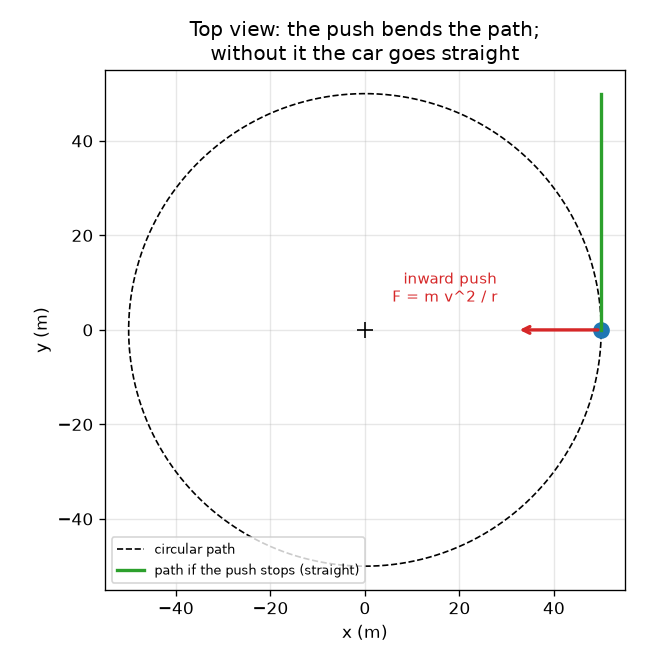
\includegraphics[width=0.85\linewidth]{figures/s01_circle_and_tangent.png}\\\small Top view: the inward push bends the path; without it the car goes straight along the tangent.\end{center}

\subsection*{E. Worked example}
A 1000 kg car drives at 10 m/s (36 km/h) round a bend of radius 50 m. Find the acceleration and the inward force, and check the effect of doubling the speed.
\begin{enumerate}[nosep]
\item a = v\textasciicircum{}2 / r = 10\textasciicircum{}2 / 50 = 100 / 50 = 2 m/s\textasciicircum{}2, pointing to the centre.
\item F = m a = 1000 * 2 = 2000 N.
\item Sanity check: the weight is m g = 1000 * 9.81 = 9810 N, so the push is about 0.2 of the weight, a gentle bend.
\item Double the speed to 20 m/s: F = 1000 * 400 / 50 = 8000 N, four times as much. Halve the radius to 25 m at 10 m/s: F = 4000 N, twice as much.
\end{enumerate}
\textbf{Answer.} a = 2 m/s\textasciicircum{}2 and F = 2000 N; doubling the speed gives 8000 N and halving the radius gives 4000 N.

\subsection*{F. Questions}
\begin{enumerate}[nosep]
\item \textbf{Conceptual.} A passenger says: 'the car pushes me outward on the bend'. Explain what is really happening, and say what the door does.
\item \textbf{Numerical.} A car of 800 kg drives at 15 m/s round a bend of radius 30 m. Find the acceleration and the inward force, and compare the force with the weight of the car.
\item \textbf{Graph and simulation interpretation.} On the graph of inward force against speed for a 1000 kg car on r = 50 m, what is the force at 10 m/s and at 20 m/s? What shape is the curve and why?
\item \textbf{Design and optimisation challenge.} Design: a 0.5 kg ball is whirled on a string of radius 0.8 m. The string breaks at 60 N. What is the largest speed you can allow, and what speed do you choose if the string should never carry more than half its breaking force?
\end{enumerate}

\section{Session 2: Friction and banking supply the inward force}

\subsection*{A. Real-world problem}
On a flat road the only thing that can push a car sideways is friction between the tyres and the road. It has a limit, and the limit is much lower on a wet road. Engineers therefore tilt (bank) fast curves so that the road itself helps to push the car inward. How fast can a car go round a flat curve of radius 100 m? What bank angle suits a curve of radius 100 m at 80 km/h? And what happens to the safe speeds when the road is wet?

\subsection*{B. Concept and theory}
Flat curve: friction supplies the inward force and cannot exceed mu N = mu m g, so m v\textasciicircum{}2 / r \textless{}= mu m g and the mass cancels: v\_max = sqrt(mu g r). Banked curve: tilt the road inward by theta. The normal force N is perpendicular to the road, so it has an inward horizontal part N sin(theta) and an upward part N cos(theta). With no friction, N cos(theta) = m g and N sin(theta) = m v\textasciicircum{}2 / r, so tan(theta) = v\textasciicircum{}2 / (g r): the ideal banking angle for speed v. With friction f along the road, at the top speed the car is about to slide up and out, so friction points down the slope with f = mu N; at the lowest speed it is about to slide down and in, so friction points up the slope. Resolving vertically and horizontally and dividing gives v\_max\textasciicircum{}2 = g r (tan(theta) + mu) / (1 - mu tan(theta)) and v\_min\textasciicircum{}2 = g r (tan(theta) - mu) / (1 + mu tan(theta)). If mu \textgreater{}= tan(theta), friction alone can hold a stopped car, so v\_min = 0. If mu tan(theta) \textgreater{}= 1, no speed makes the car slide out. The safe range is v\_min \textless{}= v \textless{}= v\_max.

\begin{itemize}[nosep]
\item mu: friction coefficient between tyre and road (dry about 0.7, wet about 0.4, ice about 0.1) (no unit)
\item g: gravitational acceleration, 9.81 (m/s\textasciicircum{}2)
\item theta: bank angle of the road, tilted towards the centre (degrees)
\item N: normal force from the road, perpendicular to its surface (N)
\item f: friction force along the road surface (N)
\item v\_max, v\_min: highest and lowest safe speed (m/s)
\end{itemize}

\begin{equation*}
v_{\max}=\sqrt{\mu g r}\quad\text{(flat curve)}
\end{equation*}

\begin{equation*}
N\cos\theta=mg,\quad N\sin\theta=\frac{mv^{2}}{r}\;\Rightarrow\;\tan\theta=\frac{v^{2}}{gr}
\end{equation*}

\begin{equation*}
N\cos\theta-s\mu N\sin\theta=mg,\quad N\sin\theta+s\mu N\cos\theta=\frac{mv^{2}}{r}\quad(s=+1\text{ top speed},\ s=-1\text{ lowest})
\end{equation*}

\begin{equation*}
v_{\max}^{2}=gr\,\frac{\tan\theta+\mu}{1-\mu\tan\theta},\qquad v_{\min}^{2}=gr\,\frac{\tan\theta-\mu}{1+\mu\tan\theta}
\end{equation*}

\begin{center}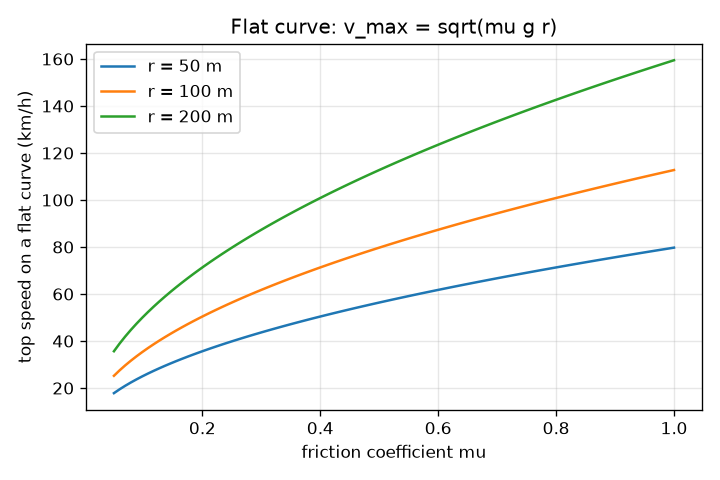
\includegraphics[width=0.85\linewidth]{figures/s02_flat_limit.png}\\\small Flat curve: top speed against friction coefficient for three radii.\end{center}

\subsection*{E. Worked example}
A curve of radius 100 m is designed for 80 km/h. Find the ideal bank angle. Then find the safe speed range on this banked curve when the road is wet with mu = 0.4.
\begin{enumerate}[nosep]
\item Convert: 80 km/h = 80 / 3.6 = 22.22 m/s.
\item tan(theta) = v\textasciicircum{}2 / (g r) = 22.22\textasciicircum{}2 / (9.81 * 100) = 493.8 / 981 = 0.5034, so theta = 26.72 degrees.
\item Top speed on the wet road: v\_max\textasciicircum{}2 = 981 * (0.5034 + 0.4) / (1 - 0.4 * 0.5034) = 981 * 0.9034 / 0.7986 = 1109.8, so v\_max = 33.31 m/s = 119.9 km/h.
\item Lowest speed: v\_min\textasciicircum{}2 = 981 * (0.5034 - 0.4) / (1 + 0.4 * 0.5034) = 981 * 0.1034 / 1.2014 = 84.4, so v\_min = 9.19 m/s = 33.1 km/h.
\item Compare with a flat wet curve: v\_max = sqrt(0.4 * 9.81 * 100) = 19.81 m/s = 71.3 km/h. Banking raises the wet limit from 71.3 to 119.9 km/h.
\end{enumerate}
\textbf{Answer.} Ideal bank angle 26.72 degrees; on that bank with mu = 0.4 the safe range is 33.1 to 119.9 km/h, against a flat-road wet limit of 71.3 km/h.

\subsection*{F. Questions}
\begin{enumerate}[nosep]
\item \textbf{Conceptual.} Why does the mass of the car not appear in v\_max = sqrt(mu g r)? Would a heavy truck and a small car have the same limit in this model?
\item \textbf{Numerical.} Find the top speed on a flat wet curve (mu = 0.4) of radius 60 m, in m/s and km/h.
\item \textbf{Graph and simulation interpretation.} On the safe-speed window graph for mu = 0.4, at what bank angle does the lowest-speed curve leave zero? What does a nonzero lowest speed mean for a slow vehicle?
\item \textbf{Design and optimisation challenge.} Design: a curve of radius 100 m has a design speed of 80 km/h and must stay safe on a wet road with mu = 0.3. Choose a bank angle. What happens if you simply use the ideal angle 26.7 degrees?
\end{enumerate}

\section{Session 3: A simulated car on a curve, checked against the formulas}

\subsection*{A. Real-world problem}
Session 2 gave formulas for the limit speed. But what really happens when a driver arrives too fast, brakes in the middle of the bend, or the road turns wet? A simulation can show the slide itself. We only trust it after it reproduces the formulas we derived and obeys energy and momentum rules. Then we can ask the engineering question: what speed limit should the sign say, with a margin for safety?

\subsection*{B. Concept and theory}
The simulation treats the car as a point mass on a road surface tilted inward by theta. State: horizontal position and velocity. Each step the normal force N follows from keeping the car on the surface, N = g cos(theta) + (v\_phi\textasciicircum{}2 / rho) sin(theta) per unit mass. The driver asks the tyres for a force along the heading (braking or accelerating, a\_long) and a sideways force to follow the lane circle of radius R, with a small steering correction when the car drifts. The friction circle limits the total tyre force: if sqrt(F\_side\textasciicircum{}2 + F\_long\textasciicircum{}2) is larger than mu N, both parts are scaled down together, so braking costs cornering grip and the car runs wide (understeer). The equations are advanced in time with the fourth-order Runge-Kutta method. Validation references: the limiting speeds of Session 2; with braking or accelerating by a on a flat road, the lateral share of the friction circle is sqrt((mu g)\textasciicircum{}2 - a\textasciicircum{}2), so the slide speed becomes sqrt(R sqrt((mu g)\textasciicircum{}2 - a\textasciicircum{}2)); a car sliding with saturated friction and no braking keeps its speed and follows a circle of radius v\textasciicircum{}2 / (mu g); with no friction, kinetic plus potential energy is conserved. A roller-coaster loop of radius r: at the top, N + m g = m v\textasciicircum{}2 / r and N \textgreater{}= 0, so v\_top \textgreater{}= sqrt(g r) and, by energy conservation over a height gain 2 r, v\_bottom \textgreater{}= sqrt(5 g r).

\begin{itemize}[nosep]
\item R: radius of the lane circle (m)
\item rho: actual distance of the car from the centre (m)
\item mu: friction coefficient (dry 0.8, wet 0.4, ice 0.1 are typical round numbers) (no unit)
\item a\_long: braking (negative) or accelerating (positive) acceleration (m/s\textasciicircum{}2)
\item dt: time step of the simulation (s)
\item ratio: tyre force asked divided by the friction limit mu N; above 1 the car slides (no unit)
\item margin: factor below the wet limit used for a speed limit sign (no unit)
\end{itemize}

\begin{equation*}
N=g\cos\theta+\frac{v_\varphi^{2}}{\rho}\sin\theta,\qquad \sqrt{F_{\mathrm{side}}^{2}+F_{\mathrm{long}}^{2}}\le \mu N\quad\text{(friction circle)}
\end{equation*}

\begin{equation*}
v_{\mathrm{slide}}(a)=\sqrt{R\sqrt{(\mu g)^{2}-a^{2}}}\quad\text{(flat road, braking or accelerating by }a)
\end{equation*}

\begin{equation*}
r_{\mathrm{skid}}=\frac{v^{2}}{\mu g}\quad\text{(radius of the path of a sliding car)}
\end{equation*}

\begin{equation*}
E=\tfrac12 v^{2}+g z=\text{constant (no friction)},\qquad v_{\mathrm{top}}\ge\sqrt{g r},\quad v_{\mathrm{bottom}}\ge\sqrt{5 g r}
\end{equation*}

\begin{center}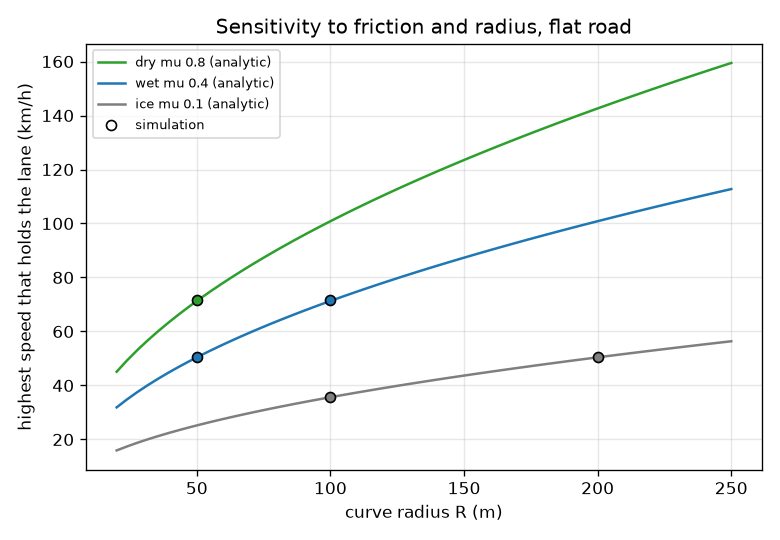
\includegraphics[width=0.85\linewidth]{figures/s03_limit_vs_radius.png}\\\small Highest speed that holds the lane against radius for dry, wet and ice roads: formula (lines) and simulation (dots).\end{center}

\subsection*{E. Worked example}
For a flat wet curve (mu = 0.4, R = 100 m) predict the top speed by hand, then find it with the simulation, and decide whether the simulation is trustworthy. Then predict where a car entering 30 percent too fast ends up after 6 s.
\begin{enumerate}[nosep]
\item Hand calculation: v = sqrt(mu g R) = sqrt(0.4 * 9.81 * 100) = 19.81 m/s = 71.3 km/h.
\item Simulation: \texttt{sim\_limit(100, 0.4, 0.0, 'max')} bisects on the start speed and gives 71.5 km/h, 0.3 percent above the formula. The small excess is because a slide that begins just above the limit takes time to grow to 1 m.
\item Banked check: for a 30 degree bank with mu = 0.3 the simulation gives 54.0 to 116.7 km/h against 54.8 to 116.2 km/h from Session 2: within 2 percent.
\item Energy check: with mu = 0 on a 20 degree bank the energy per kg stays constant to better than 1e-13 (relative), so the integrator does not create or destroy energy.
\item Failure case: entering at 1.3 times the limit, 92.7 km/h = 25.75 m/s, the car slides on a circle of radius v\textasciicircum{}2 / (mu g) = 25.75\textasciicircum{}2 / 3.924 = 169.0 m. After 6 s it is at (34.2, 133.9) m in the simulation and at (34.2, 133.9) m on the analytic circle: 138.2 m from the centre, far outside a lane of radius 100 m.
\end{enumerate}
\textbf{Answer.} Hand 71.3 km/h, simulation 71.5 km/h (within 0.3 percent); the car entering at 1.3 times the limit slides on a circle of radius 169 m and is 138 m from the centre after 6 s.

\subsection*{F. Questions}
\begin{enumerate}[nosep]
\item \textbf{Conceptual.} Why does braking in the middle of a bend make a slide more likely, even though braking reduces the speed?
\item \textbf{Numerical.} A road with mu = 0.4 has a flat curve of radius 100 m. Find the speed at which a car accelerating at 2 m/s\textasciicircum{}2 loses grip. Compare with the speed without acceleration.
\item \textbf{Graph and simulation interpretation.} In the radius graph, the dry, wet and ice lines are curves that rise with radius. By what factor does the limit change if the radius is multiplied by 4, and if mu is divided by 4 (wet to ice)?
\item \textbf{Design and optimisation challenge.} Design: a loop of a roller coaster has radius 10 m. What minimum speed is needed at the top and at the bottom? Choose a design speed at the bottom with a 10 percent margin and say what the passengers feel at the top.
\end{enumerate}

\section{Real-world mini-project}
\textbf{Set the speed limit sign for a curve.} A council asks you to choose the speed limit sign for a curve of radius 80 m, banked at 4 degrees, whose wet surface has a friction coefficient of 0.35. The sign must leave a safety margin on the wet limit and be a multiple of 5 km/h. Use \texttt{analytic\_limits}, \texttt{posted\_speed\_limit} and \texttt{holds} from Session 3, compare margins of 0.6, 0.7, 0.75, 0.8 and 0.9, and check each sign speed in the simulation on a wet road and on ice (mu 0.1).

\section{The path ahead}
\begin{enumerate}[nosep]
\item \textbf{Session 4: Transition spiral into the curve.} A path made of a straight, a clothoid and an arc, followed by the Session 3 car.
\item \textbf{Session 5: Weight transfer between left and right wheels.} A car with centre of gravity height, track width and four tyre loads.
\item \textbf{Session 6: Rollover before sliding.} A rollover check added to the friction-circle limit.
\item \textbf{Session 7: Plan the speed round a whole circuit.} A speed planner for a stadium circuit of two 100 m straights and two half circles of radius 30 m.
\item \textbf{Session 8: Measure mu and compare with a turntable.} A short lab report with a measured mu, a predicted slip speed and a measured slip speed.
\end{enumerate}

\section{Answers and hints}

\subsection*{Session 1}
\begin{enumerate}[nosep]
\item \textbf{Conceptual.} Hint: Think about what the passenger's body would do if nothing pushed it, and which object pushes the passenger inward. Solution: Nothing pushes the passenger outward. By inertia the body tends to keep moving in a straight line at constant velocity. The car turns inward, so the door (and the seat) moves toward the passenger and presses inward on the body, giving it the inward acceleration v\textasciicircum{}2 / r. The passenger feels that contact force from the door and interprets it as being thrown outward. If the door were open, the passenger would move straight along the tangent, which is away from the centre but not along the radius.
\item \textbf{Numerical.} Hint: a = v\textasciicircum{}2 / r first, then F = m a; weight = m g with g = 9.81 m/s\textasciicircum{}2. Solution: a = 15\textasciicircum{}2 / 30 = 225 / 30 = 7.5 m/s\textasciicircum{}2. F = 800 * 7.5 = 6000 N. Weight = 800 * 9.81 = 7848 N, so F is about 0.76 of the weight. Sanity check: units are m\textasciicircum{}2/s\textasciicircum{}2 divided by m, which is m/s\textasciicircum{}2, and kg * m/s\textasciicircum{}2 is N. A push of 0.76 of the weight is a very sharp bend: ordinary tyres on dry road can only supply about 0.7 to 0.9 of the weight, so this is close to the limit.
\item \textbf{Graph and simulation interpretation.} Hint: Use F = m v\textasciicircum{}2 / r for each speed and compare the two values. Solution: At 10 m/s the force is 2000 N (2 kN); at 20 m/s it is 8000 N (8 kN). The curve is a parabola, because F is proportional to the square of v: doubling v multiplies F by 4. The curve for twice the radius lies below it at half the height at every speed.
\item \textbf{Design and optimisation challenge.} Hint: Solve F = m v\textasciicircum{}2 / r for v = sqrt(F r / m) with the allowed force. Solution: At the breaking force: v = sqrt(60 * 0.8 / 0.5) = sqrt(96) = 9.80 m/s. With a safety margin of half the breaking force, 30 N: v = sqrt(30 * 0.8 / 0.5) = sqrt(48) = 6.93 m/s. The margin costs about 29 percent of the speed, because v grows only with the square root of F. When the string breaks, the ball moves off along the tangent in a straight line.
\end{enumerate}

\subsection*{Session 2}
\begin{enumerate}[nosep]
\item \textbf{Conceptual.} Hint: Write the inward force needed and the largest friction force, and see what happens to m. Solution: The inward force needed is m v\textasciicircum{}2 / r and the largest friction force is mu m g (N = m g on a flat road). Both are proportional to m, so m cancels and the limit depends only on mu, g and r. In this simple model a truck and a small car with the same tyres and road have the same limit. Real trucks differ because they can tip over, their load shifts and their tyres behave differently, none of which is in the model.
\item \textbf{Numerical.} Hint: v = sqrt(mu g r). Solution: v = sqrt(0.4 * 9.81 * 60) = sqrt(235.4) = 15.34 m/s. In km/h: 15.34 * 3.6 = 55.2 km/h. Sanity check: the 100 m curve gives 71.3 km/h and the speed goes with the square root of the radius, so the 60 m curve should give 71.3 * sqrt(0.6) = 55.2 km/h. It does.
\item \textbf{Graph and simulation interpretation.} Hint: The lowest speed is zero while friction alone can hold a stopped car: mu \textgreater{}= tan(theta). Solution: The curve leaves zero where tan(theta) = mu = 0.4, that is theta = 21.8 degrees. Above this angle a stopped or slow vehicle slides down the bank towards the inside of the curve, because gravity along the slope exceeds the friction that the road can give. On the same graph with mu = 0.7 the angle is 35.0 degrees.
\item \textbf{Design and optimisation challenge.} Hint: The smallest angle that keeps 80 km/h at or below the top speed is tan(theta) = (k - mu) / (1 + mu k) with k = v\textasciicircum{}2 / (g r). Then compute the lowest speed for the steeper angle. Solution: k = 0.5034, so tan(theta) = (0.5034 - 0.3) / (1 + 0.3 * 0.5034) = 0.1767 and theta = 10.02 degrees; a bank of 10 degrees gives a wet top speed of 79.96 km/h, just below 80, so choose 12 degrees (top speed 83.4 km/h) or 15 degrees (88.6 km/h) for a margin. With the ideal angle 26.7 degrees the wet top speed is 109.7 km/h but the lowest speed becomes 47.4 km/h, so slow traffic or a stopped car on a wet or icy road would slide inward. Trade-off: a steeper bank raises the top speed but also raises the lowest safe speed. Assumptions: one mu, point-mass car, no margin for tipping.
\end{enumerate}

\subsection*{Session 3}
\begin{enumerate}[nosep]
\item \textbf{Conceptual.} Hint: Think of the friction circle: the tyre force has a fixed budget mu N to share between braking and cornering. Solution: The tyres can give a total force of at most mu N. Braking uses part of that budget, so less is left for the sideways force. For a car at the lane circle the sideways demand is v\textasciicircum{}2 / R, which falls only as the speed falls. At the moment the driver brakes, the demand is the full sideways demand plus the braking demand: the total can exceed mu N. In the simulation a car entering at 0.9 of the limit has a demand ratio of 0.81 when coasting but 1.11 when braking at 3 m/s\textasciicircum{}2. Brake before the bend, not in it.
\item \textbf{Numerical.} Hint: v\_slide = sqrt(R * sqrt((mu g)\textasciicircum{}2 - a\textasciicircum{}2)). Solution: mu g = 0.4 * 9.81 = 3.924 m/s\textasciicircum{}2. (mu g)\textasciicircum{}2 = 15.40, a\textasciicircum{}2 = 4, difference 11.40, square root 3.376 m/s\textasciicircum{}2 (the lateral budget). v = sqrt(100 * 3.376) = 18.37 m/s = 66.1 km/h. Without acceleration the limit is 71.3 km/h, so accelerating at 2 m/s\textasciicircum{}2 lowers the limit by about 5 km/h. The simulation gives 66.2 km/h.
\item \textbf{Graph and simulation interpretation.} Hint: The limit is sqrt(mu g R). Solution: The limit is proportional to the square root of R and to the square root of mu. Four times the radius doubles the limit; a quarter of the friction halves it. So a wet road (0.4) that goes to ice (0.1) loses half of its limit speed: from 71.3 to 35.7 km/h at R = 100 m. The dots from the simulation follow the same lines.
\item \textbf{Design and optimisation challenge.} Hint: v\_top = sqrt(g r); energy: v\_bottom\textasciicircum{}2 = v\_top\textasciicircum{}2 + 4 g r. Solution: v\_top = sqrt(9.81 * 10) = 9.90 m/s; v\_bottom = sqrt(5 * 9.81 * 10) = 22.15 m/s (79.7 km/h). With a 10 percent margin on the bottom speed: 24.4 m/s. The margin makes the top speed sqrt(24.4\textasciicircum{}2 - 4 * 98.1) = 14.2 m/s, with N = m (v\textasciicircum{}2 / r - g) = m * (20.15 - 9.81) = 10.3 m, about 1.05 times the weight: passengers feel pressed into their seats with about 1.05 times their body weight. Assumptions: no friction or air drag, a point mass, and a perfect circle (real loops are not circular because the force would jump).
\end{enumerate}

\section{How to join}
Read \texttt{CONTRIBUTING.md} in the repository, then pick an issue labelled \texttt{good first issue}. Repository: \url{https://github.com/KrunalPanchal1995/opencentripetal}

\end{document}
